\chapter{Arsitektur Frontend Berskala Besar}
\label{ch:frontend}

\section*{Tujuan Pembelajaran}
\begin{itemize}
  \item Membedakan \textit{server state} dari \textit{client state} pada satu
        halaman, lalu menyebut akibatnya pada ukuran halaman dan pada
        perilakunya saat berpindah.
  \item Mengukur biaya hidrasi penuh dan hidrasi selektif pada halaman yang
        sama, lalu menunjukkan bagian mana yang tumbuh mengikuti besar
        halaman.
  \item Merancang \textit{application shell} beserta \textit{routing}, batas
        \textit{error}, dan \textit{progressive enhancement}-nya, lalu
        membuktikan isinya tetap tampil ketika skripnya tidak jalan.
\end{itemize}

\section{Pendahuluan}

Bab 8 memilih tempat HyperText Markup Language (HTML) dirakit, dan Bab 5
mengukur apa yang terjadi sesudah HTML itu tiba. Bab ini menggarap bagian yang menghubungkan keduanya,
yaitu susunan kode di sisi \textit{frontend} ketika halamannya tidak lagi
kecil: batas antarkomponen, tempat \textit{state} disimpan, dan berapa banyak
pekerjaan yang masih harus dikerjakan browser sesudah HTML tampil.

Pekerjaan sesudah HTML tampil itu disebut hidrasi (\textit{hydration}).
Server mengirim HTML yang sudah berisi, lalu skrip di browser menghidupkan
bagian-bagiannya agar dapat diklik dan diketik. Pertanyaan yang menentukan
biayanya cuma satu: berapa banyak bagian yang dihidupkan. Menghidupkan
seluruh halaman dan menghidupkan dua kotak saja menghasilkan tampilan yang
sama persis di mata pengguna, tetapi tidak menghasilkan biaya yang sama.

Demonya satu halaman katalog yang dilayani dalam tiga varian: dua cara
hidrasi dan satu \textit{application shell} beserta \textit{routing}-nya.
Referensi utamanya adalah HTML Standard untuk \textit{form}, skrip, dan
riwayat sesi \cite{whatwg-html}, dokumentasi Astro untuk gagasan \textit{island}
\cite{astro-islands}, dokumentasi React untuk hidrasi HTML yang dikirim server
\cite{react-hydrateroot}, dan WCAG 2.2 untuk syarat aksesibilitasnya
\cite{w3c-wcag22}.

\section{Batas Komponen dan Komposisi}

Komponen adalah satu bagian halaman yang punya batas jelas: ia menerima data,
mengembalikan tampilan, dan tidak menyentuh apa pun di luar dirinya. Pada
demo bab ini tiap komponen adalah satu fungsi yang mengembalikan potongan
HTML. Komponen besar disusun dari komponen kecil, dan susunan itulah yang
disebut komposisi.

Analoginya seperti bangunan yang dirakit dari beton pracetak. Tiap panel
dicetak terpisah dengan ukuran yang sudah pasti, lalu dipasang di tempatnya.
Panel yang rusak dapat diganti satu buah, dan tidak ada yang perlu
membongkar dindingnya.

Gambar \ref{fig:komposisi} memperlihatkan susunan komponen pada halaman
katalog tersebut.

\begin{figure}[!htb]
  \centering
  \begin{tikzpicture}[
    font=\scriptsize,
    kotak/.style={draw, rounded corners, minimum height=0.8cm,
                  minimum width=2.1cm, align=center, font=\scriptsize\bfseries},
    panah/.style={-{Stealth[length=2mm]}, thick}
  ]
    \node[kotak, fill=praditagreen!15] (halaman) at (0,2.1) {tata\_letak\\{\tiny\mdseries kerangka halaman}};
    \node[kotak, fill=orange!12] (penyaring) at (-3.4,0.9) {penyaring\\{\tiny\mdseries pulau}};
    \node[kotak, fill=orange!12] (keranjang) at (-0.9,0.9) {keranjang\\{\tiny\mdseries pulau}};
    \node[kotak, fill=blue!8] (daftar) at (2.4,0.9) {daftar\_buku\\{\tiny\mdseries 1 buah}};
    \node[kotak, fill=blue!8] (kartu) at (2.4,-0.4) {kartu\_buku\\{\tiny\mdseries 200 buah}};
    \node[kotak, fill=blue!8] (tombol) at (2.4,-1.7) {tombol Tambah\\{\tiny\mdseries 200 buah}};

    \draw[panah] (halaman) -| (penyaring);
    \draw[panah] (halaman) -| (keranjang);
    \draw[panah] (halaman) -| (daftar);
    \draw[panah] (daftar) -- (kartu);
    \draw[panah] (kartu) -- (tombol);
    \node[font=\tiny, gray, anchor=west] at (3.6,-0.4) {menerima satu buku};
    \node[font=\tiny, gray, anchor=west] at (3.6,0.9) {menerima daftar buku};
  \end{tikzpicture}
  \caption{Susunan komponen halaman katalog pada halaman berisi 200 buku}
  \label{fig:komposisi}
\end{figure}

Dua contoh ukuran dari susunan tersebut:
\begin{enumerate}
  \item Pada halaman berisi 200 buku, atribut \texttt{data-komponen} muncul
        403 kali: satu daftar, 200 kartu, 200 tombol, satu penyaring, dan
        satu keranjang.
  \item Atribut \texttt{data-pulau} hanya muncul dua kali, yaitu pada
        penyaring dan pada keranjang, dan jumlah itu tidak berubah walaupun
        bukunya menjadi 2.000.
\end{enumerate}

Listing \ref{lst:komponen11} memperlihatkan komponen terkecilnya. Kartu
menerima satu buku dan mengembalikan HTML-nya, tanpa tahu ada berapa kartu
lain di halaman yang sama.

\begin{lstlisting}[style=PythonStyle, caption={Komponen terkecil menerima satu buku dan mengembalikan HTML, tersedia di \berkas{sources/chapter11/komponen.py}}, label={lst:komponen11}]
def kartu_buku(buku):
  """Menyusun satu kartu buku, yaitu komponen terkecil pada halaman ini.

  Atribut data-komponen dipakai skrip hidrasi penuh untuk menemukan seluruh
  bagian yang perlu dihidupkan, sehingga jumlahnya dapat dihitung.
  """
  judul = html.escape(buku["judul"])
  harga = f"Rp {buku['harga']:,}".replace(",", ".")
  alamat = f"/kerangka/buku/{buku['id']}"
  return (
      f'      <li class="kartu" data-komponen="kartu"'
      f' data-id="{buku["id"]}">\n'
      f'        <a class="judul" href="{alamat}">{judul}</a>\n'
      f'        <span class="harga">{harga}</span>\n'
      '        <button data-komponen="tombol" type="button">'
      "Tambah</button>\n"
      "      </li>"
  )
\end{lstlisting}

Batas yang jelas itu punya satu akibat yang langsung terasa pada bab ini.
Karena tiap komponen menandai dirinya, jumlah komponen di satu halaman dapat
dihitung dengan satu perintah, dan biaya menghidupkannya dapat diukur, bukan
dikira-kira.

\section{Design System dan Token}

\textit{Design system} adalah kumpulan keputusan tampilan yang disepakati
sekali lalu dipakai berulang: warna, jarak, ukuran huruf, dan bentuk
komponen. Bentuk paling sederhananya adalah token, yaitu nilai bernama yang
disimpan di satu tempat \cite{dtcg-format}.

Analoginya seperti satu kaleng cat untuk seluruh gedung. Selama warnanya
diambil dari kaleng yang sama, dinding di lantai tiga tidak akan berbeda tipis
dari dinding di lantai satu. Begitu ada yang mencampur sendiri, perbedaannya
muncul dan tidak ada yang tahu mana yang benar.

Tabel \ref{tab:token} memuat token yang dipakai demo bab ini beserta tempat
pemakaiannya.

\begin{table}[!htb]
  \centering
  \caption{Token \textit{design system} pada demo bab ini}
  \label{tab:token}
  \begin{tabularx}{\textwidth}{llX}
    \hline
    \textbf{Token} & \textbf{Nilai} & \textbf{Dipakai pada} \\
    \hline
    \texttt{warna\_utama} & \#257147 & judul buku \\
    \hline
    \texttt{warna\_teks} & \#1a1a1a & seluruh teks halaman \\
    \hline
    \texttt{warna\_garis} & \#d8d8d8 & garis tepi kartu \\
    \hline
    \texttt{jarak\_kecil} & 4px & jarak antarkartu \\
    \hline
    \texttt{jarak\_sedang} & 12px & jarak di dalam kartu \\
    \hline
    \texttt{lebar\_halaman} & 720px & lebar maksimum badan halaman \\
    \hline
  \end{tabularx}
\end{table}

Listing \ref{lst:token11} memperlihatkan keenam token itu sebagai satu
sumber nilai. Komponen tidak menulis angka tampilan sendiri, dan gaya halaman
dibentuk dari token tersebut.

\begin{lstlisting}[style=PythonStyle, caption={Token sebagai satu sumber nilai tampilan, tersedia di \berkas{sources/chapter11/komponen.py}}, label={lst:token11}]
TOKEN = {
    "warna_utama": "#257147",
    "warna_teks": "#1a1a1a",
    "warna_garis": "#d8d8d8",
    "jarak_kecil": "4px",
    "jarak_sedang": "12px",
    "lebar_halaman": "720px",
}
\end{lstlisting}

Keuntungannya terlihat saat ada perubahan. Mengubah satu baris di
\texttt{TOKEN} mengubah seluruh halaman sekaligus, dan tidak ada tempat lain
yang perlu dicari. Pada proyek yang besar, token inilah yang membuat dua tim
yang bekerja terpisah tetap menghasilkan tampilan yang sama.

\section{Server State lawan Client State}

\textit{State} adalah data yang menentukan tampilan saat ini. Dua jenis
\textit{state} pada aplikasi web sering tertukar. Pembagiannya begini.
\textit{Server state} dimiliki server, misalnya daftar buku beserta harganya,
dan browser hanya memegang \textit{copy}-nya. \textit{Client state} lahir dan mati di
browser, misalnya kata yang sedang diketik di kotak penyaring.

Analoginya seperti papan pengumuman jurusan. Isi pengumumannya milik jurusan,
dan siapa pun yang memotretnya hanya memegang \textit{copy}. Catatan kecil yang
ditempel seseorang di buku agendanya sendiri adalah hal yang lain: tidak ada
di papan, dan hilang bersama agendanya.

Gambar \ref{fig:state} memperlihatkan pembagian itu pada demo bab ini,
beserta jalan yang ditempuh masing-masing.

\begin{figure}[!htb]
  \centering
  \begin{tikzpicture}[
    font=\scriptsize,
    kotak/.style={draw, rounded corners, minimum height=0.9cm,
                  minimum width=2.6cm, align=center, font=\scriptsize\bfseries},
    panah/.style={-{Stealth[length=2mm]}, thick}
  ]
    \node[kotak, fill=praditagreen!15] (server) at (0,0) {Server\\{\tiny\mdseries daftar buku, harga, stok}};
    \node[kotak, fill=blue!8] (html) at (4.3,0.9) {HTML berisi\\{\tiny\mdseries 200 kartu tercetak}};
    \node[kotak, fill=orange!12] (blok) at (4.3,-0.9) {Blok state\\{\tiny\mdseries JSON di halaman}};
    \node[kotak, fill=green!10] (browser) at (8.6,0) {Browser\\{\tiny\mdseries saringan, keranjang}};

    \draw[panah] (server.east) -- ++(0.3,0) |- (html.west);
    \draw[panah] (server.east) -- ++(0.3,0) |- (blok.west);
    \draw[panah] (html.east) -- ++(0.3,0) |- (browser.west);
    \draw[panah] (blok.east) -- ++(0.3,0) |- (browser.west);
    \node[font=\tiny, gray, anchor=north] at (4.3,-1.5) {hanya diperlukan bila komponen dibangun ulang};
  \end{tikzpicture}
  \caption{\textit{Server state} tiba dua kali: sebagai HTML yang sudah
           tercetak, dan sebagai blok \textit{state} untuk hidrasi}
  \label{fig:state}
\end{figure}

Gambar tersebut memuat masalah yang menjadi inti bab ini. Pada varian hidrasi
penuh, data buku tiba dua kali: sekali sebagai HTML yang sudah tercetak, dan
sekali lagi sebagai JSON (JavaScript Object Notation) di dalam blok
\textit{state}. Pengiriman kedua itulah yang membuat halaman 200 buku tumbuh
dari 55.674 byte menjadi 71.950 byte, naik 16.276 byte atau 29 persen.

\textit{Client state} menanggung akibat yang berbeda, dan akibatnya terlihat
saat berpindah halaman. Angka keranjang pada demo ini disimpan di dalam DOM
(Document Object Model), yaitu di satu elemen di halaman. Begitu wilayah itu
diganti, angkanya kembali ke nol. \textit{State} yang harus bertahan melewati
perpindahan tidak boleh tinggal di bagian yang ikut diganti.

\section{Server Component lawan Client Component}

Pembagian \textit{state} di atas punya pasangannya di sisi kode.
\textit{Server component} dirender di server, tidak ikut terunduh sebagai
JavaScript, dan boleh menyentuh basis data. \textit{Client component}
diunduh, berjalan di browser, dan hanya karena itulah ia dapat menyimpan
\textit{state} serta menanggapi peristiwa \cite{react-server-components}.

Demo bab ini memakai pembagian yang sama tanpa \textit{framework}. Kartu,
daftar, dan tombol dirender di server. Penyaring dan keranjang ditandai
sebagai pulau, yaitu satu-satunya bagian yang memang perlu hidup di browser
\cite{astro-islands}. Tabel \ref{tab:komponen-sisi} memuat pembagiannya
beserta jumlah yang benar-benar dihidupkan pada kedua varian.

\begin{table}[!htb]
  \centering
  \caption{Pembagian komponen dan jumlah yang dihidupkan pada halaman 200
           buku, hasil pengukuran nyata}
  \label{tab:komponen-sisi}
  \begin{tabularx}{\textwidth}{Xlll}
    \hline
    \textbf{Komponen} & \textbf{Jumlah} & \textbf{Hidrasi penuh} & \textbf{Hidrasi selektif} \\
    \hline
    kartu buku & 200 & dihidupkan & tidak \\
    \hline
    tombol Tambah & 200 & dihidupkan & tidak \\
    \hline
    daftar & 1 & dihidupkan & tidak \\
    \hline
    penyaring & 1 & dihidupkan & dihidupkan \\
    \hline
    keranjang & 1 & dihidupkan & dihidupkan \\
    \hline
    \textbf{Jumlah dihidupkan} & & \textbf{403} & \textbf{2} \\
    \hline
  \end{tabularx}
\end{table}

Pembagian itu menentukan \textit{state} apa yang perlu dikirim. Listing
\ref{lst:state11} memperlihatkan keduanya berdampingan: yang pertama membawa
data seluruh buku, yang kedua tidak membawa data buku sama sekali.

\begin{lstlisting}[style=PythonStyle, caption={State yang dikirim kedua varian, tersedia di \berkas{sources/chapter11/komponen.py}}, label={lst:state11}]
def state_penuh(daftar):
  """Menyusun state yang dikirim bila seluruh komponen akan dihidupkan.

  Hidrasi penuh membangun ulang tiap komponen di browser, dan untuk itu ia
  butuh data tiap komponen. Karena itu data seluruh kartu ikut dikirim di
  dalam halaman, selain sudah tercetak sebagai HTML.
  """
  return {
      "buku": {str(buku["id"]): buku for buku in daftar},
      "keranjang": 0,
      "saringan": "",
  }


def state_pulau():
  """Menyusun state yang dikirim bila hanya pulau yang akan dihidupkan.

  Pulau tidak membangun ulang kartu, sehingga data kartu tidak diperlukan di
  browser. Yang tersisa hanya milik kedua pulau itu sendiri.
  """
  return {"keranjang": 0, "saringan": ""}
\end{lstlisting}

Tombol Tambah menunjukkan bahwa jumlah komponen yang dihidupkan bukan takdir.
Varian penuh memasang satu \textit{listener} di tiap tombol, sehingga 200
tombol berarti 200 \textit{listener}. Varian selektif memasang satu
\textit{listener} di daftarnya, lalu memeriksa sendiri tombol mana yang
diklik. Perilakunya sama, dan hal itu sudah diperiksa di browser: pada kedua
varian, dua klik menaikkan angka keranjang menjadi 2.

\section{Hidrasi Penuh lawan Hidrasi Selektif}

Hidrasi penuh menghidupkan seluruh komponen di halaman, termasuk kartu yang
tidak pernah disentuh pengguna \cite{react-hydrateroot}. Hidrasi selektif
hanya menghidupkan bagian yang ditandai sebagai pulau, dan sisa halaman tetap
menjadi HTML kiriman server \cite{astro-islands}. Gambar \ref{fig:hidrasi}
memperlihatkan perbedaan jangkauannya.

\begin{figure}[!htb]
  \centering
  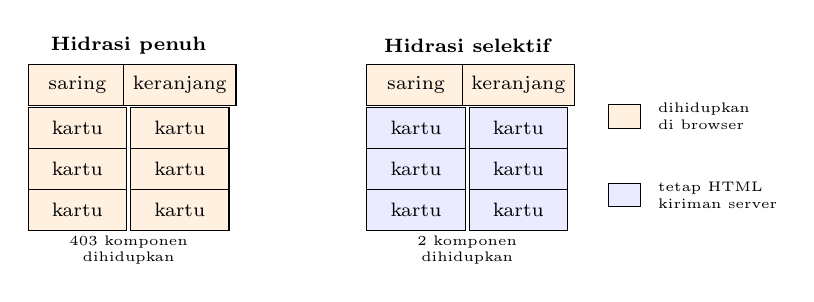
\begin{tikzpicture}[
    font=\scriptsize,
    sel/.style={draw, minimum height=0.52cm, minimum width=1.25cm},
    judul/.style={font=\scriptsize\bfseries, align=center},
    panah/.style={-{Stealth[length=2mm]}, thick}
  ]
    \node[judul] at (1.3,1.5) {Hidrasi penuh};
    \node[sel, fill=orange!12] at (0.65,1.0) {saring};
    \node[sel, fill=orange!12] at (1.95,1.0) {keranjang};
    \foreach \y in {0.45,-0.07,-0.59} {
      \node[sel, fill=orange!12] at (0.65,\y) {kartu};
      \node[sel, fill=orange!12] at (1.95,\y) {kartu};
    }
    \node[font=\tiny, align=center] at (1.3,-1.1) {403 komponen\\dihidupkan};

    \node[judul] at (5.6,1.5) {Hidrasi selektif};
    \node[sel, fill=orange!12] at (4.95,1.0) {saring};
    \node[sel, fill=orange!12] at (6.25,1.0) {keranjang};
    \foreach \y in {0.45,-0.07,-0.59} {
      \node[sel, fill=blue!8] at (4.95,\y) {kartu};
      \node[sel, fill=blue!8] at (6.25,\y) {kartu};
    }
    \node[font=\tiny, align=center] at (5.6,-1.1) {2 komponen\\dihidupkan};

    \node[sel, fill=orange!12, minimum width=0.4cm, minimum height=0.3cm] at (7.6,0.6) {};
    \node[font=\tiny, anchor=west, align=left] at (7.9,0.6) {dihidupkan\\di browser};
    \node[sel, fill=blue!8, minimum width=0.4cm, minimum height=0.3cm] at (7.6,-0.4) {};
    \node[font=\tiny, anchor=west, align=left] at (7.9,-0.4) {tetap HTML\\kiriman server};
  \end{tikzpicture}
  \caption{Jangkauan hidrasi pada halaman yang sama berisi 200 buku}
  \label{fig:hidrasi}
\end{figure}

Kedua skrip berangkat dari baris yang hampir sama, dan selisihnya hanya pada
apa yang dicari di halaman. Listing \ref{lst:hidrasi11} memperlihatkan
keduanya.

\begin{lstlisting}[language=TypeScript, caption={Satu baris pembeda: yang dicari komponen atau pulau, tersedia di \berkas{sources/chapter11/statis/}}, label={lst:hidrasi11}]
function hidrasiPenuh() {
  const mulai = performance.now();
  const state = bacaState();
  const daftar = document.querySelectorAll("[data-komponen]");
  for (const node of daftar) {
    hidupkanKomponen(node, state);
  }
  laporkan(daftar.length, performance.now() - mulai);
}

function hidrasiSelektif() {
  const mulai = performance.now();
  const state = bacaState();
  const daftar = document.querySelectorAll("[data-pulau]");
  for (const node of daftar) {
    hidupkanPulau(node, state);
  }
  laporkan(daftar.length, performance.now() - mulai);
}
\end{lstlisting}

Halaman mengukur dirinya sendiri dengan \texttt{performance.now()}, lalu
menuliskan hasilnya ke halaman. Pengukurannya diulang lima kali untuk tiap
varian pada tiga besar halaman, dan yang dicatat adalah nilai tengahnya.
Tabel \ref{tab:hidrasi} memuat seluruh hasilnya.

\begin{table}[!htb]
  \centering
  \caption{Biaya hidrasi kedua varian pada tiga besar halaman, hasil
           pengukuran nyata}
  \label{tab:hidrasi}
  \begin{tabularx}{\textwidth}{Xlllll}
    \hline
    \textbf{Buku} & \textbf{Varian} & \textbf{Komponen} & \textbf{HTML byte} & \textbf{Tengah ms} & \textbf{Rentang ms} \\
    \hline
    200 & penuh & 403 & 71.950 & 1,50 & 1,20--2,10 \\
    \hline
    200 & selektif & 2 & 55.674 & 0,50 & 0,50--0,70 \\
    \hline
    1.000 & penuh & 2.003 & 358.360 & 3,90 & 3,60--4,70 \\
    \hline
    1.000 & selektif & 2 & 275.679 & 1,00 & 0,60--1,00 \\
    \hline
    2.000 & penuh & 4.003 & 722.356 & 7,10 & 6,30--10,40 \\
    \hline
    2.000 & selektif & 2 & 553.677 & 0,80 & 0,70--0,90 \\
    \hline
  \end{tabularx}
\end{table}

Tabel itu punya dua konsekuensi praktis. Pertama, biaya hidrasi penuh tumbuh
mengikuti jumlah komponen: 1,50 milidetik pada 403 komponen, lalu 7,10
milidetik pada 4.003 komponen. Kedua, biaya hidrasi selektif tidak bergerak
dan tetap di bawah satu milidetik, karena yang dihidupkan tetap dua, berapa
pun bukunya.

Satu kejanggalan di tabel itu layak dijelaskan. Angka varian selektif tidak
urut: 1,00 milidetik pada 1.000 buku, lalu 0,80 milidetik pada 2.000 buku.
Urutan terbalik itu bukan kesalahan baca, melainkan tanda bahwa biayanya
sudah sekecil \textit{noise} pengukurannya. Yang tersisa untuk diukur hanya
pencarian kedua pulaunya dan dua pemasangan \textit{listener}, dan keduanya
tidak bertambah ketika bukunya bertambah. Rentang varian penuh justru lebar
di baris terakhir, 6,30 sampai 10,40 milidetik, karena pengukuran di satu
komputer ikut menanggung pekerjaan lain yang sedang berjalan.

Angka milidetik di tabel itu kecil, dan kekecilannya jangan buru-buru
disimpulkan. Pengukurannya berjalan di komputer meja; pada telepon kelas
bawah, pekerjaan JavaScript yang sama lazim beberapa kali lebih lambat.
Selisih ukuran halaman justru lebih mudah dirasakan. Pada halaman 2.000 buku,
blok \textit{state} tambahannya 168.679 byte, dan pada sambungan 1,5 Mbit per
detik, byte sebanyak itu memakan sekitar 0,9 detik sebelum satu baris skrip
pun berjalan.

\section{Application Shell, Routing, dan Strategi Pengambilan Data}

\textit{Application shell} adalah bagian halaman yang tidak berubah saat
pengguna berpindah: judul, navigasi, dan kerangka tata letaknya. Yang
berpindah hanya isi satu wilayah. \textit{Routing} di sisi browser bertugas
mengganti isi wilayah itu tanpa memuat ulang dokumen, dan menjaga alamat di
bilah alamat tetap benar \cite{whatwg-html}.

Analoginya seperti ruang kuliah dengan satu papan tulis. Dinding, meja, dan
pintunya tidak dibongkar tiap kali mata kuliahnya berganti. Yang dihapus dan
ditulis ulang hanya papannya.

Gambar \ref{fig:kerangka} memperlihatkan pembagian itu beserta alamat yang
diambil router pada tiap perpindahan.

\begin{figure}[!htb]
  \centering
  \begin{tikzpicture}[
    font=\scriptsize,
    kotak/.style={draw, rounded corners, minimum height=0.75cm,
                  minimum width=3.0cm, align=center, font=\scriptsize\bfseries},
    panah/.style={-{Stealth[length=2mm]}, thick}
  ]
    \node[kotak, fill=praditagreen!15, minimum width=5.2cm] (judul) at (0,1.5) {Judul dan navigasi\\{\tiny\mdseries dikirim sekali, tidak dimuat ulang}};
    \node[kotak, fill=orange!12, minimum width=5.2cm, minimum height=1.5cm] (wilayah) at (0,0.1) {Wilayah\\{\tiny\mdseries isinya diganti tiap perpindahan}};
    \node[kotak, fill=blue!8] (fragmen) at (6.4,0.1) {/fragmen/buku/3\\{\tiny\mdseries 217 byte}};
    \node[font=\tiny, align=center, fill=gray!35, rounded corners, inner sep=2pt] (dokumen) at (6.4,1.5) {/kerangka/buku/3\\dokumen penuh, 1.071 byte};

    \draw[panah] (fragmen) -- (wilayah);
    \draw[panah, dashed] (dokumen.west) -- ++(-0.5,0) |- (judul.east);
    \node[font=\tiny, gray, anchor=north, align=center] at (0,-1.1) {kerangka dikirim sekali, lalu hanya wilayahnya yang diganti};
  \end{tikzpicture}
  \caption{\textit{Application shell}: kerangka tetap, wilayahnya diganti
           dengan fragmen}
  \label{fig:kerangka}
\end{figure}

Listing \ref{lst:rute11} memperlihatkan inti routernya. Dua hal diperiksa
sekaligus, yaitu kegagalan jaringan lewat \texttt{try} dan kegagalan di
server lewat status responsnya.

\begin{lstlisting}[language=TypeScript, caption={Mengambil fragmen, lalu memasangnya sebagai isi wilayah, tersedia di \berkas{sources/chapter11/statis/rute.js}}, label={lst:rute11}]
async function muatWilayah(alamat) {
  try {
    const respon = await fetch(alamatFragmen(alamat));
    if (!respon.ok) {
      tampilkanGagal(PESAN_GAGAL);
      return;
    }
    document.getElementById("wilayah").innerHTML = await respon.text();
  } catch (gagal) {
    tampilkanGagal(PESAN_GAGAL);
  }
}
\end{lstlisting}

Pertanyaan kemudian muncul: seberapa besar penghematannya. Tabel
\ref{tab:rute} memuat ukuran dokumen penuh dan ukuran fragmen untuk tujuan
yang sama, diukur pada halaman 200 buku.

\begin{table}[!htb]
  \centering
  \caption{Ukuran dokumen penuh lawan ukuran fragmen untuk tujuan yang sama,
           hasil pengukuran nyata}
  \label{tab:rute}
  \begin{tabularx}{\textwidth}{Xllll}
    \hline
    \textbf{Tujuan} & \textbf{Status} & \textbf{Dokumen} & \textbf{Fragmen} & \textbf{Fragmen \%} \\
    \hline
    \texttt{/katalog} & 200 & 55.943 & 55.089 & 98,5 \\
    \hline
    \texttt{/katalog?saring=jaringan} & 200 & 10.414 & 9.560 & 91,8 \\
    \hline
    \texttt{/buku/3} & 200 & 1.071 & 217 & 20,3 \\
    \hline
    \texttt{/gagal} & 500 & 1.023 & 169 & 16,5 \\
    \hline
  \end{tabularx}
\end{table}

Baris pertama tabel itu sengaja dibiarkan apa adanya, walaupun melawan
harapan. Fragmen katalog 98,5 persen sebesar dokumennya, karena isi yang
dituju memang hampir seluruh halaman. Penghematan baru terasa pada tujuan
yang kecil: fragmen halaman satu buku 217 byte, sedangkan dokumennya 1.071
byte.

Angka 1.071 byte itu pun belum lengkap. Dokumen membawa kerangka, gaya, dan
rujukan ke \berkas{rute.js} yang berukuran 4.188 byte, dan skrip itu harus
diurai serta dijalankan ulang tiap kali dokumennya dimuat. Perpindahan lewat
fragmen tidak menyentuh satu pun dari ketiganya. Itulah yang sebenarnya
dihemat \textit{routing} di sisi browser, dan penghematan itu tidak muncul di
kolom byte.

Strategi pengambilan datanya mengikuti pembagian yang sama. Wilayah pertama
dirender server, sehingga halaman langsung berisi pada permintaan pertama.
Perpindahan berikutnya mengambil fragmen. Hasilnya sudah diperiksa di
browser: tautan "Buku 3" mengganti isi wilayah tanpa memuat ulang dokumen,
alamat di bilah alamat berubah menjadi \texttt{/kerangka/buku/3}, dan tombol
kembali browser memulihkan katalog beserta 200 barisnya.

\section{Batas Error, Progressive Enhancement, dan Aksesibilitas}

Batas \textit{error} adalah kesepakatan bahwa kegagalan satu bagian tidak
membuat seluruh halaman ikut gagal. Bagian yang gagal diganti pesan, dan sisanya
tetap dapat dipakai. Pada demo bab ini, alamat \texttt{/kerangka/gagal}
sengaja menjawab 500, dan router menggantinya dengan satu pesan.

Hasilnya sudah diperiksa di browser. Ketika wilayah gagal dimuat, keempat
tautan navigasi tetap ada, dokumen tidak dimuat ulang, dan perpindahan
berikutnya tetap jalan. Tanpa batas tersebut, satu permintaan yang gagal akan
meninggalkan wilayah kosong tanpa keterangan apa-apa.

\textit{Progressive enhancement} adalah urutan membangunnya: HTML yang sudah
berfungsi lebih dahulu, lalu skrip menambah kenyamanan di atasnya. Listing
\ref{lst:pe11} memperlihatkan penyaring yang dibangun dengan urutan itu.
Bentuk dasarnya \textit{form} biasa yang dikirim ke server.

\begin{lstlisting}[style=PythonStyle, caption={Penyaring sebagai form yang sudah jalan tanpa skrip, tersedia di \berkas{sources/chapter11/komponen.py}}, label={lst:pe11}]
def penyaring(saringan):
  """Menyusun penyaring sebagai form biasa, bukan sebagai kotak yang kosong.

  Form dengan metode GET sudah berfungsi sebelum satu baris JavaScript pun
  berjalan: penekanan tombol Saring mengirim ulang permintaan, dan server
  yang menyaring. Pulau penyaring hanya mempercepatnya menjadi tanpa muat
  ulang. Itulah bentuk progressive enhancement yang paling murah.
  """
  nilai = html.escape(saringan)
  return (
      '    <form class="penyaring" method="get" action="">\n'
      '      <label for="saring">Saring judul</label>\n'
      f'      <input id="saring" name="saring" value="{nilai}"\n'
      '        data-pulau="penyaring" data-komponen="penyaring" />\n'
      '      <button type="submit">Saring</button>\n'
      "    </form>"
  )
\end{lstlisting}

Klaim "tetap jalan tanpa skrip" pantas diuji, bukan dipercaya. Pengujiannya
membuka tiap halaman dua kali dengan Chrome tanpa jendela: sekali seperti
biasa, sekali dengan CSP (Content Security Policy) yang menolak seluruh
skrip, sehingga halaman terlihat seperti ketika file JavaScript-nya gagal
diunduh. Tabel \ref{tab:tanpa-js} memuat jumlah baris katalog yang terpasang
di DOM pada keduanya.

\begin{table}[!htb]
  \centering
  \caption{Isi yang tetap tampil ketika skripnya diblokir, hasil pengukuran
           nyata pada halaman 200 buku}
  \label{tab:tanpa-js}
  \begin{tabularx}{\textwidth}{Xlll}
    \hline
    \textbf{Halaman} & \textbf{Skrip jalan} & \textbf{Skrip mati} & \textbf{Form} \\
    \hline
    \texttt{/selektif} & 200 baris & 200 baris & ada \\
    \hline
    \texttt{/selektif?saring=jaringan} & 33 baris & 33 baris & ada \\
    \hline
    \texttt{/kerangka/katalog} & 200 baris & 200 baris & ada \\
    \hline
    \texttt{/kerangka/katalog?saring=jaringan} & 33 baris & 33 baris & ada \\
    \hline
  \end{tabularx}
\end{table}

Kedua kolom angkanya sama, dan kesamaan itulah hasilnya: tidak ada satu baris
katalog pun yang bergantung pada skrip. Penyaringannya pun tetap bekerja,
karena server yang menyaring, dan 33 baris itu adalah jumlah buku yang
judulnya memuat kata "jaringan". Yang hilang tanpa skrip hanya kenyamanannya:
penyaringan menempuh satu permintaan baru, dan perpindahan halaman memuat
ulang dokumen.

Aksesibilitas mengikuti urutan yang sama, dan sebagian besarnya didapat
cuma-cuma. Tombol Tambah adalah \texttt{<button>} sungguhan, sehingga dapat
dicapai dengan tombol Tab dan ditekan dengan spasi. Kotak penyaring punya
\texttt{<label for>}, sehingga pembaca layar menyebutkan namanya. Tautan
navigasi adalah \texttt{<a href>} dengan alamat sungguhan, sehingga dapat
dibuka di tab baru walaupun routernya ada. Wilayah yang isinya berubah
ditandai \texttt{aria-live="polite"}, agar penggantian isinya ikut
diberitakan \cite{w3c-wcag22}.

\section{Ringkasan}

Komponen dan token mengatur kode, bukan biaya. Keduanya tetap penting karena
batas yang jelas membuat halaman dapat dihitung: pada halaman 200 buku, demo
bab ini memuat 403 komponen bertanda dan dua pulau, dan angka itu didapat
dengan satu perintah. Token membuat nilai tampilan punya satu sumber,
sehingga satu baris cukup untuk mengubah seluruh halaman.

Yang mengatur biaya adalah pembagian \textit{state} dan jangkauan hidrasinya.
Hidrasi penuh menghidupkan 403 komponen dalam 1,50 milidetik, dan pada
halaman 2.000 buku menghidupkan 4.003 komponen dalam 7,10 milidetik. Hidrasi
selektif menghidupkan dua pulau dalam 0,50 sampai 1,00 milidetik, berapa pun
bukunya. Angkanya bahkan tidak urut menurut besar halaman, dan ketidakurutan
itu menunjukkan biayanya sudah sekecil \textit{noise} pengukurannya.

Selisih yang lebih mudah dirasakan pengguna justru ada di ukuran halaman.
Hidrasi penuh menuntut data tiap komponen dikirim ulang sebagai JSON,
sehingga halaman 2.000 buku membawa 168.679 byte tambahan, atau 30 persen
lebih besar. Pada sambungan lambat, byte sebanyak itu memakan sekitar 0,9
detik sebelum hidrasinya dimulai.

\textit{Application shell} memisahkan yang tetap dari yang berganti.
Perpindahan ke halaman satu buku mengambil 217 byte, bukan 1.071 byte
dokumen beserta 4.188 byte skripnya. Penghematannya tidak selalu besar:
fragmen katalog 98,5 persen sebesar dokumennya, karena yang dituju memang
hampir seluruh halaman. Keuntungan yang selalu didapat bukan byte, melainkan
kerangka yang tidak dibangun ulang dan skrip yang tidak dijalankan ulang.

Pesan utama bab ini adalah urutan membangunnya. HTML yang sudah berfungsi
diletakkan paling bawah, lalu skrip ditambahkan hanya pada bagian yang
memang butuh hidup. Dengan urutan itu, halaman 200 buku tetap menampilkan 200
baris dan penyaringnya tetap bekerja walaupun seluruh skripnya diblokir, dan
satu wilayah yang gagal tidak membawa serta sisa halamannya.

\section{Latihan}

Seluruh file yang dipakai pada latihan ini tersedia di
\berkas{sources/chapter11/}, dihitung relatif terhadap akar repositori.
Latihan ini membutuhkan Python 3 dan satu browser berbasis Chromium, tanpa
Docker dan tanpa pustaka tambahan.

Seluruh permintaan diarahkan ke aplikasi yang berjalan di komputer sendiri,
dan sifatnya mengamati, bukan membebani. Angka milidetik tiap mahasiswa akan
berbeda, karena bergantung pada komputernya. Yang dilaporkan adalah pola
perbandingannya, bukan angka persisnya.

Penyiapannya satu perintah, seperti pada Listing \ref{lst:c11-siapkan}.

\begin{lstlisting}[language=bash, caption={Menyalakan aplikasi katalog, tersedia di \berkas{sources/chapter11/aplikasi.py}}, label={lst:c11-siapkan}]
cd sources/chapter11
python3 aplikasi.py &

# Keluarannya:
# Melayani di http://127.0.0.1:8080/penuh dengan 200 buku  (Ctrl+C untuk berhenti)
\end{lstlisting}

\subsection*{Latihan 1: Menghitung Komponen dan Biaya State}

Latihan ini membuktikan bahwa jumlah pulau tidak tumbuh mengikuti besar
halaman, sedangkan jumlah komponen dan ukuran halaman tumbuh.

\begin{enumerate}
  \item Nyalakan aplikasi dengan jumlah buku bawaan, lalu hitung kemunculan
        \texttt{data-komponen} dan \texttt{data-pulau} pada kedua varian,
        seperti pada Listing \ref{lst:c11-lat1-jalan}.
  \item Catat ukuran HTML kedua varian, lalu hitung selisihnya.
  \item Hentikan aplikasi, nyalakan ulang dengan
        \texttt{JUMLAH\_BUKU=1000}, lalu ulangi kedua langkah di atas.
  \item Isi Tabel \ref{tab:c11-lat1-hasil}. Tabel \ref{tab:c11-lat1-contoh}
        memperlihatkan contoh yang sudah terisi.
  \item Jawab dua pertanyaan berikut. Pertama, berapa persen tambahan ukuran
        HTML pada varian penuh, dan dari mana asalnya? Kedua, mengapa jumlah
        pulau tetap dua walaupun bukunya lima kali lebih banyak?
\end{enumerate}

\begin{lstlisting}[language=bash, caption={Menghitung komponen dan ukuran halaman, tersedia di \berkas{sources/chapter11/aplikasi.py}}, label={lst:c11-lat1-jalan}]
curl -s http://127.0.0.1:8080/penuh | grep -c 'data-komponen='
curl -s http://127.0.0.1:8080/selektif | grep -c 'data-pulau='
curl -s http://127.0.0.1:8080/penuh | wc -c
curl -s http://127.0.0.1:8080/selektif | wc -c

# Keluarannya:
# 403
# 2
# 71950
# 55674
\end{lstlisting}

\begin{table}[!htb]
  \centering
  \caption{Contoh hasil Latihan 1 yang sudah terisi}
  \label{tab:c11-lat1-contoh}
  \begin{tabularx}{\textwidth}{Xllll}
    \hline
    \textbf{Buku} & \textbf{Komponen} & \textbf{Pulau} & \textbf{HTML penuh} & \textbf{HTML selektif} \\
    \hline
    200 & 403 & 2 & 71.950 & 55.674 \\
    \hline
    1.000 & 2.003 & 2 & 358.360 & 275.679 \\
    \hline
  \end{tabularx}
\end{table}

\begin{table}[!htb]
  \centering
  \caption{Lembar isian hasil pengukuran Latihan 1}
  \label{tab:c11-lat1-hasil}
  \begin{tabularx}{\textwidth}{Xllll}
    \hline
    \textbf{Buku} & \textbf{Komponen} & \textbf{Pulau} & \textbf{HTML penuh} & \textbf{HTML selektif} \\
    \hline
    200 & \dots & \dots & \dots & \dots \\
    \hline
    1.000 & \dots & \dots & \dots & \dots \\
    \hline
  \end{tabularx}
\end{table}

\subsection*{Latihan 2: Biaya Hidrasi Dua Varian}

Latihan ini mengukur biaya hidrasi kedua varian pada tiga besar halaman, lalu
memisahkan bagian yang tumbuh dari bagian yang tetap.

\begin{enumerate}
  \item Jalankan \berkas{ukur-hidrasi.py} pada jumlah buku bawaan, seperti
        pada Listing \ref{lst:c11-lat2-jalan}.
  \item Hentikan aplikasi, nyalakan ulang dengan
        \texttt{JUMLAH\_BUKU=1000}, lalu ukur sekali lagi. Ulangi untuk
        \texttt{JUMLAH\_BUKU=2000}.
  \item Isi Tabel \ref{tab:c11-lat2-hasil}. Tabel \ref{tab:c11-lat2-contoh}
        memperlihatkan contoh yang sudah terisi.
  \item Buka kedua varian di browser, yaitu \texttt{/penuh} dan
        \texttt{/selektif} pada port 8080, lalu bandingkan baris laporan di
        bawah judul halamannya.
  \item Jawab tiga pertanyaan berikut. Pertama, bagian mana yang tumbuh
        mengikuti besar halaman, dan bagian mana yang tidak? Kedua, mengapa
        angka varian selektif tidak urut menurut besar halaman? Ketiga, pada
        besar halaman berapa selisihnya mulai pantas dipersoalkan, dan dengan
        alasan apa?
\end{enumerate}

\begin{lstlisting}[language=bash, caption={Mengukur biaya hidrasi lima kali tiap varian, tersedia di \berkas{sources/chapter11/ukur-hidrasi.py}}, label={lst:c11-lat2-jalan}]
python3 ukur-hidrasi.py

# Keluarannya:
#   Varian     Buku  Komponen  HTML byte  JS byte  Tengah ms   Rentang ms
#   penuh       200       403      71950     3723       1.50    1.20-2.10
#   selektif    200         2      55674     3278       0.50    0.50-0.70
\end{lstlisting}

\begin{table}[!htb]
  \centering
  \caption{Contoh hasil Latihan 2 yang sudah terisi}
  \label{tab:c11-lat2-contoh}
  \begin{tabularx}{\textwidth}{Xllll}
    \hline
    \textbf{Buku} & \textbf{Penuh, ms} & \textbf{Selektif, ms} & \textbf{Komponen penuh} & \textbf{Pulau} \\
    \hline
    200 & 1,50 & 0,50 & 403 & 2 \\
    \hline
    1.000 & 3,90 & 1,00 & 2.003 & 2 \\
    \hline
    2.000 & 7,10 & 0,80 & 4.003 & 2 \\
    \hline
  \end{tabularx}
\end{table}

\begin{table}[!htb]
  \centering
  \caption{Lembar isian hasil pengukuran Latihan 2}
  \label{tab:c11-lat2-hasil}
  \begin{tabularx}{\textwidth}{Xllll}
    \hline
    \textbf{Buku} & \textbf{Penuh, ms} & \textbf{Selektif, ms} & \textbf{Komponen penuh} & \textbf{Pulau} \\
    \hline
    200 & \dots & \dots & \dots & \dots \\
    \hline
    1.000 & \dots & \dots & \dots & \dots \\
    \hline
    2.000 & \dots & \dots & \dots & \dots \\
    \hline
  \end{tabularx}
\end{table}

\subsection*{Latihan 3: Biaya Perpindahan pada Kerangka}

Latihan ini membandingkan biaya satu perpindahan lewat fragmen dengan biaya
memuat dokumen penuh, lalu memeriksa perilaku kerangkanya di browser.

\begin{enumerate}
  \item Jalankan \berkas{ukur-rute.py}, seperti pada Listing
        \ref{lst:c11-lat3-jalan}, lalu catat keempat barisnya.
  \item Buka \texttt{http://127.0.0.1:8080/kerangka/katalog} di browser,
        tekan tautan "Buku 3", lalu perhatikan alamat di bilah alamat dan
        bagian halaman yang berubah.
  \item Tekan tombol kembali browser, lalu catat apakah katalognya pulih.
  \item Tekan tombol Tambah dua kali, lalu pindah ke halaman buku dan
        kembali lagi. Catat angka keranjangnya sesudah kembali.
  \item Isi Tabel \ref{tab:c11-lat3-hasil}. Tabel \ref{tab:c11-lat3-contoh}
        memperlihatkan contoh yang sudah terisi.
  \item Jawab tiga pertanyaan berikut. Pertama, mengapa fragmen katalog
        hampir sebesar dokumennya? Kedua, apa yang tetap dihemat perpindahan
        lewat fragmen walaupun selisih bytenya kecil? Ketiga, mengapa angka
        keranjang kembali ke nol, dan di mana seharusnya \textit{state} itu
        disimpan?
\end{enumerate}

\begin{lstlisting}[language=bash, caption={Membandingkan ukuran dokumen dan fragmen, tersedia di \berkas{sources/chapter11/ukur-rute.py}}, label={lst:c11-lat3-jalan}]
python3 ukur-rute.py

# Keluarannya:
#   Tujuan                    Status   Dokumen   Fragmen  Fragmen %
#   /katalog                 200/200     55943     55089      98.5%
#   /katalog?saring=jaringan 200/200     10414      9560      91.8%
#   /buku/3                  200/200      1071       217      20.3%
#   /gagal                   500/500      1023       169      16.5%
\end{lstlisting}

\begin{table}[!htb]
  \centering
  \caption{Contoh hasil Latihan 3 yang sudah terisi}
  \label{tab:c11-lat3-contoh}
  \begin{tabularx}{\textwidth}{Xll}
    \hline
    \textbf{Hal yang diamati} & \textbf{Hasil} & \textbf{Keterangan} \\
    \hline
    Fragmen \texttt{/buku/3} & 217 byte & dokumennya 1.071 byte \\
    \hline
    Fragmen \texttt{/katalog} & 55.089 byte & 98,5 persen dari dokumennya \\
    \hline
    Alamat sesudah menekan tautan & \texttt{/kerangka/buku/3} & tanpa muat ulang \\
    \hline
    Tombol kembali browser & katalog pulih & 200 baris \\
    \hline
    Keranjang sesudah kembali & 0 & disimpan di DOM wilayah \\
    \hline
  \end{tabularx}
\end{table}

\begin{table}[!htb]
  \centering
  \caption{Lembar isian hasil pengamatan Latihan 3}
  \label{tab:c11-lat3-hasil}
  \begin{tabularx}{\textwidth}{Xll}
    \hline
    \textbf{Hal yang diamati} & \textbf{Hasil} & \textbf{Keterangan} \\
    \hline
    Fragmen \texttt{/buku/3} & \dots & \dots \\
    \hline
    Fragmen \texttt{/katalog} & \dots & \dots \\
    \hline
    Alamat sesudah menekan tautan & \dots & \dots \\
    \hline
    Tombol kembali browser & \dots & \dots \\
    \hline
    Keranjang sesudah kembali & \dots & \dots \\
    \hline
  \end{tabularx}
\end{table}

\subsection*{Latihan 4: Apa yang Tersisa Tanpa Skrip}

Latihan ini membuktikan bahwa isi katalog dan penyaringnya tidak bergantung
pada JavaScript, dan memperlihatkan batas \textit{error} menahan satu wilayah
yang gagal.

\begin{enumerate}
  \item Jalankan \berkas{ukur-tanpa-js.py}, seperti pada Listing
        \ref{lst:c11-lat4-jalan}, lalu catat keempat barisnya.
  \item Buka \texttt{http://127.0.0.1:8080/kerangka/katalog?blokir\_skrip=1}
        di browser, ketik "jaringan" di kotak penyaring, lalu tekan tombol
        Saring. Catat jumlah baris yang tersisa dan apakah halamannya dimuat
        ulang.
  \item Buka alamat yang sama tanpa \texttt{blokir\_skrip}, lalu ulangi
        penyaringan yang sama. Catat perbedaannya.
  \item Tekan tautan "Bagian yang gagal", lalu catat apa yang tampil di
        wilayah dan apakah navigasinya masih utuh.
  \item Isi Tabel \ref{tab:c11-lat4-hasil}. Tabel \ref{tab:c11-lat4-contoh}
        memperlihatkan contoh yang sudah terisi.
  \item Jawab tiga pertanyaan berikut. Pertama, bagian mana yang hilang
        tanpa skrip, dan bagian mana yang tetap? Kedua, apa yang akan terlihat
        di halaman ini bila katalognya dirakit di browser seperti varian SPA
        (Single-Page Application) pada Bab 8? Ketiga, mengapa router
        memeriksa status responsnya, bukan cuma menangkap kegagalan jaringan?
\end{enumerate}

\begin{lstlisting}[language=bash, caption={Memeriksa isi yang tetap tampil tanpa skrip, tersedia di \berkas{sources/chapter11/ukur-tanpa-js.py}}, label={lst:c11-lat4-jalan}]
python3 ukur-tanpa-js.py

# Keluarannya:
#   Halaman                            Skrip jalan Skrip mati  Form
#   /selektif                                  200        200   ada
#   /selektif?saring=jaringan                   33         33   ada
#   /kerangka/katalog                          200        200   ada
#   /kerangka/katalog?saring=jaringan           33         33   ada
\end{lstlisting}

\begin{table}[!htb]
  \centering
  \caption{Contoh hasil Latihan 4 yang sudah terisi}
  \label{tab:c11-lat4-contoh}
  \begin{tabularx}{\textwidth}{Xll}
    \hline
    \textbf{Hal yang diamati} & \textbf{Skrip jalan} & \textbf{Skrip mati} \\
    \hline
    Baris katalog & 200 & 200 \\
    \hline
    Baris sesudah disaring & 33 & 33 \\
    \hline
    Cara penyaringan & tanpa muat ulang & satu permintaan baru \\
    \hline
    Wilayah yang gagal & diganti pesan & halaman 500 dari server \\
    \hline
    Navigasi sesudah gagal & utuh, 4 tautan & utuh, 4 tautan \\
    \hline
  \end{tabularx}
\end{table}

\begin{table}[!htb]
  \centering
  \caption{Lembar isian hasil pengamatan Latihan 4}
  \label{tab:c11-lat4-hasil}
  \begin{tabularx}{\textwidth}{Xll}
    \hline
    \textbf{Hal yang diamati} & \textbf{Skrip jalan} & \textbf{Skrip mati} \\
    \hline
    Baris katalog & \dots & \dots \\
    \hline
    Baris sesudah disaring & \dots & \dots \\
    \hline
    Cara penyaringan & \dots & \dots \\
    \hline
    Wilayah yang gagal & \dots & \dots \\
    \hline
    Navigasi sesudah gagal & \dots & \dots \\
    \hline
  \end{tabularx}
\end{table}
